\documentclass[journal, table]{IEEEtran}
\usepackage[english, spanish]{babel}
\usepackage[sorting=none]{biblatex}
\bibliography{ref.bib}
\usepackage{amsmath, amsfonts, amsthm}
\usepackage{hyperref, url}
\hyphenation{op-tical net-works semi-conduc-tor}
\usepackage{graphicx}
\usepackage{float}
\usepackage{fancyhdr, last page}
\usepackage{siunitx}
\usepackage{anyfontsize}
\usepackage{csquotes}
\usepackage{svg}
\usepackage{tabularx, ragged2e, booktabs}
\usepackage{xcolor}
\usepackage{multirow}
\usepackage{adjustbox}
\usepackage[affil-sl]{authblk}
\usepackage[electronic]{ifsym}
\usepackage{tikz}
\usepackage[spanish]{cleveref}
\usepackage{circuitikz}
\usetikzlibrary{patterns}
\usepackage{scalerel}
\usepackage{pict2e}
\usepackage{tkz-euclide}
\usetikzlibrary{calc}
\usetikzlibrary{arrows.meta}
\usetikzlibrary{shadows}
\usetikzlibrary{external}
\usetikzlibrary{decorations.pathmorphing}
\usetikzlibrary{shapes.geometric}
\usetikzlibrary{arrows,shapes.gates.logic.US,shapes.gates.logic.IEC,calc}
\usepackage{pgfplots}
\pgfplotsset{compat=newest}
\usepgfplotslibrary{statistics}
\usepgfplotslibrary{fillbetween}

\AtBeginDocument{\decimalpoint}

\hypersetup{
	colorlinks=true,
	linkcolor=black,
	urlcolor=blue,
	pdftitle={Flip-flops-JLAB}
}
\urlstyle{same}
\sisetup{separate-uncertainty}

\begin{document}
\tikzstyle{branch}=[fill,shape=circle,minimum size=3pt, inner sep=0pt]

\title{\textbf{Flip-flops} \\ \small{ }}

\author[*]{Julian Avila
	\thanks{Julian Avila: 20212107030}}
\author[*]{Laura Herrera
	\thanks{Laura Herrera: 20212107011}}
\author[*]{Bryan Martínez
	\thanks{Bryan Martínez: 20212107008}}
\author[*]{Juan Acuña
	\thanks{Juan Acuña: 20212107034}}

\affil[*]{Proyecto Curricular de Física \\ Universidad Distrital Francisco José de Caldas}

\date{2024-05-15}

\markboth{}
{Shell \MakeLowercase{\textit{et al.}}: Bare Demo of IEEEtran.cls for IEEE Journals}

\maketitle

\section{Construcción de Flip-Flop de forma discreta}
\subsection{Montaje y tabla de verdad}
Se construyó un flip-flop JK aparir del uso de compuertas NAND y OR con entradas negadas.
La \Cref{fig:discrete-jk} muestra el diagrama del circuito lógico como también
el detector de flanco derecho para la señal de reloj.
El detector permite que el flip-flop cambie de estado solo cuando la señal de
reloj presente un aumento, esto se puede evidenciar con la \Cref{fig:jk-signal}.

\begin{figure}[h!]
	\centering
	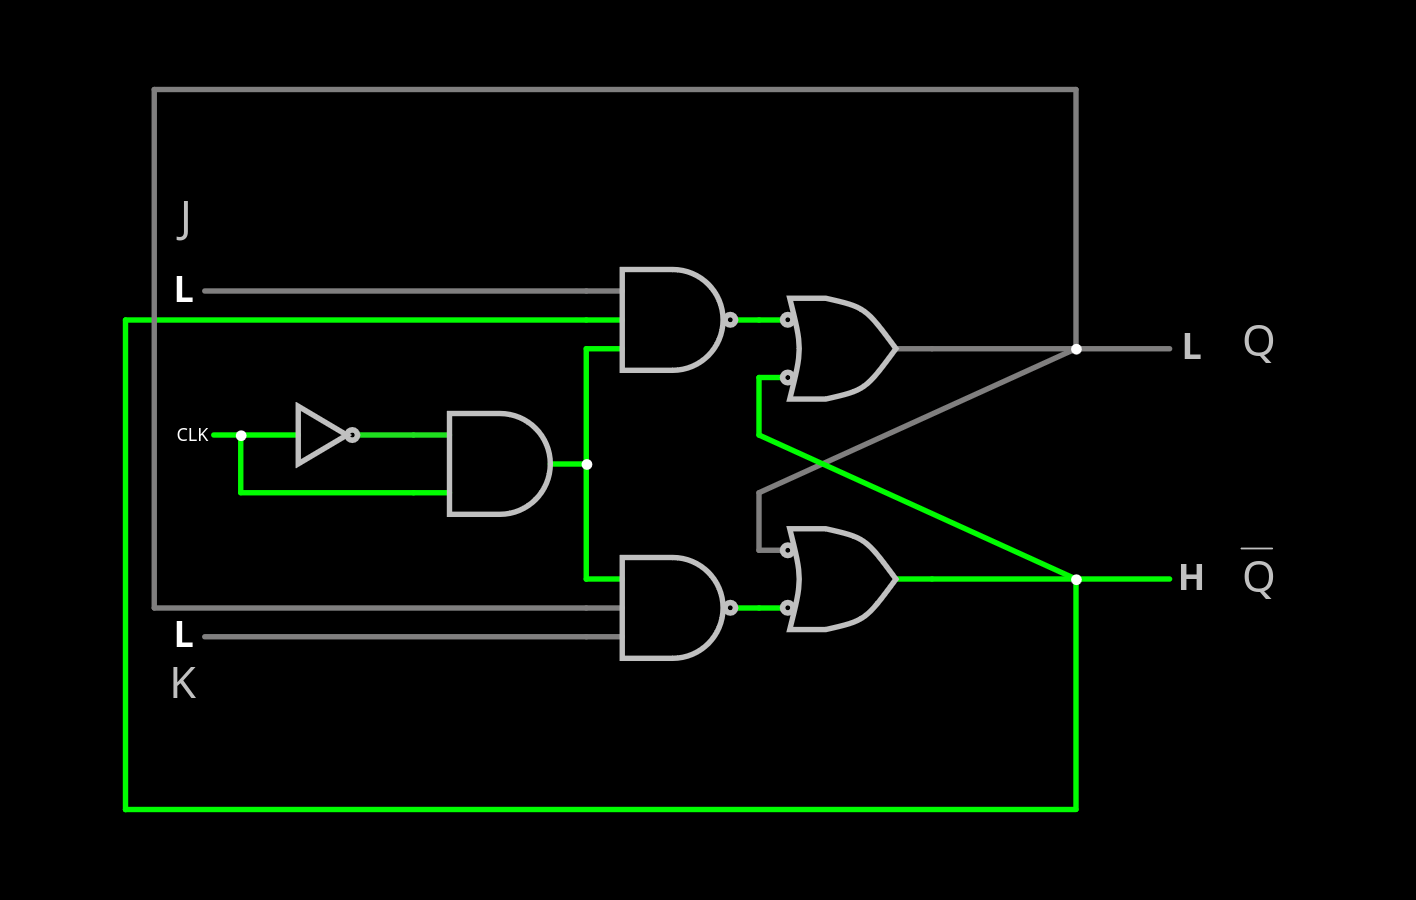
\includegraphics[width=0.8\linewidth]{./Discrete-FF/ff-jk-circuit.png}
	\caption{Diagrama del flip-flop jk construido de forma discreta.}
	\label{fig:discrete-jk}
\end{figure}

\begin{figure}[h!]
	\centering
	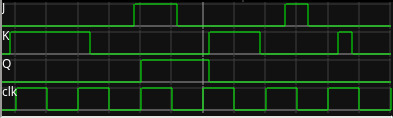
\includegraphics[width=0.8\linewidth]{./Discrete-FF/oscilloscope.jpeg}
	\caption{Señal tomada del osciloscopio.}
	\label{fig:jk-signal}
\end{figure}

A partir del montaje se obtuvieron los resultados que se presentan en el
\Cref{tab:discrete-jk} de forma simplificada.

\begin{table}[h!]
	\centering
	\rowcolors{2}{white}{gray!25}
	\begin{tabular}{c|c|c||c|c}
		\toprule
		CLK & J & K & Q & $\bar{\text{Q}}$ \\
		\midrule
		\RaisingEdge & 0 & 0 & $\text{Q}_{0}$ & $\bar{\text{Q}}_{0}$ \\
		\RaisingEdge & 0 & 1 & 0 & 1 \\
		\RaisingEdge & 1 & 0 & 1 & 0 \\
		\RaisingEdge & 1 & 1 & $\bar{\text{Q}}_{0}$ & $\text{Q}_{0}$ \\
		\bottomrule
	\end{tabular}
	\caption{Tabla de resultados. (Simplificada)}
	\label{tab:discrete-jk}
\end{table}

\subsection{Análisis de resultados}

\subsection{Conclusiones}

\printbibliography
\nocite{*}

\end{document}
